For the results shown in Chapter~\ref{chap:HPROMResults}, all simulations have simply \textit{reconstructed} the training data. That is, the geometry, initial conditions, boundary conditions, and simulation duration of each PROM are identical to those of the FOM from which the training data are extracted. Although these simulations were successful in this effort, the ultimate goal of any data-driven method is \textit{generalizability}. To be truly useful for engineering applications, such methods must be able to make fast and accurate predictions for unseen configurations which are not accounted for in the training data. 

\section{Failure of Static Trial Bases}

The PROMs investigated in Chapter~\ref{chap:HPROMResults} are, unfortunately, not generalizable. To demonstrate this for the truncated CVRC case examined in Section~\ref{sec:cvrc}, the unsampled MP-LSVT PROM is allowed to run for a longer duration than the original FOM training data, to $\timeVar = 5.6$ ms. The resulting dump plane corner pressure probe is shown in Fig.~\ref{fig:cvrcStaticFutureState}. Even though the PROM is capable of simulating the training period with exceptionally high accuracy, the solution rapidly deviates shortly after the end of the training period at $\timeVar = 5.5$ ms. The dominant cause of this failure is the inability of the linear trial space to model realizations of the flow field which were not included in the training data. In a sense, this is an attempt at \textit{extrapolation} in time (rather than a sort of \textit{interpolation} within the training set). Although disappointing, this result is not at all surprising, as data-driven methods often struggle to model unseen data, particularly for highly non-linear systems.

\begin{figure}
    \begin{minipage}{0.45\linewidth}
        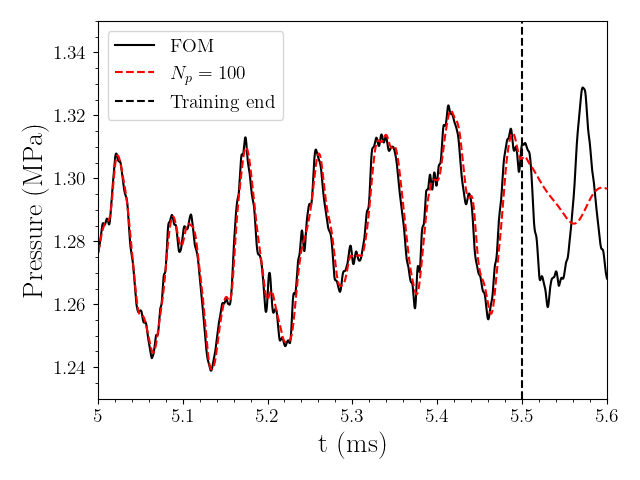
\includegraphics[width=0.99\linewidth]{Chapters/AdaptiveResults/Images/cvrc/pressure_probe_static_future.png}
        \caption{\label{fig:cvrcStaticFutureState}CVRC pressure probe, unsampled MP-LSVT, $\numPrimModes = 100$, $\dt = 5 \times \dtFOM$.}
    \end{minipage}
    \hspace{0.5em}
    \begin{minipage}{0.45\linewidth}
        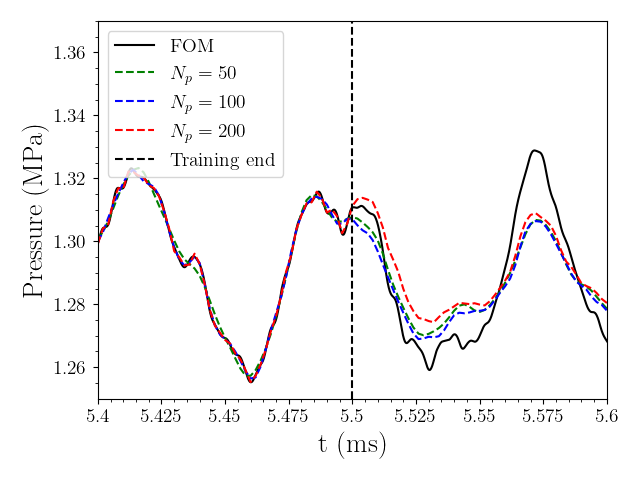
\includegraphics[width=0.99\linewidth]{Chapters/AdaptiveResults/Images/cvrc/pressure_probe_projection.png}
        \caption{\label{fig:cvrcStaticProjProbe}CVRC pressure probe, projected solution, various $\numPrimModes$.}
    \end{minipage}
\end{figure}

The inability of the trial basis to represent unseen data is made readily apparent by observing the average projection error over time in Fig.~\ref{fig:cvrcStaticProjTime}. After $\timeVar = 5.5$ ms, the projection error drastically increases, and increasing the dimension of the trial basis is unable to improve this whatsoever. This can be visually observed in pressure probe measurements of the projected solution in Fig.~\ref{fig:cvrcStaticProjProbe}, where large discrepancies can be observed beyond $\timeVar = 5.5$ ms. 

\begin{figure}
    \centering
    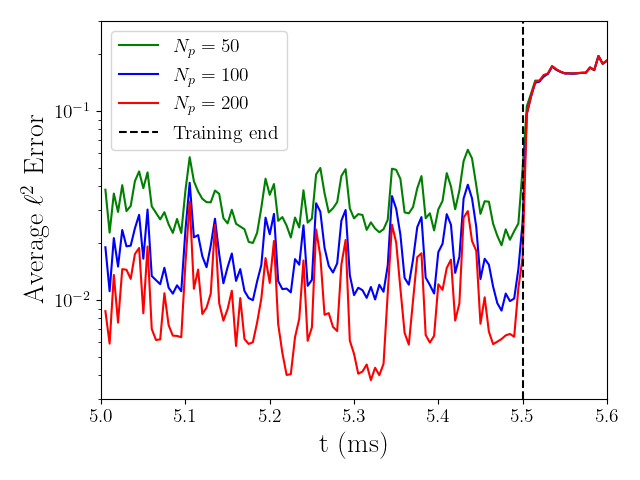
\includegraphics[width=0.75\linewidth]{Chapters/AdaptiveResults/Images/cvrc/proj_err_time.png}
    \caption{\label{fig:cvrcStaticProjTime}CVRC average projection error over time, various $\numPrimModes$.}
\end{figure}

Comparisons of the FOM and projected pressure and temperature fields at $\timeVar = 5.6$ ms can be seen in Figs.~\ref{fig:cvrcStaticPressureProjSlice} and~\ref{fig:cvrcStaticTempProjSlice}. In both instances, the solution appears smeared and more axisymmetric, lacking most of the transient features of the flow field such as the  highly distorted flame front in the combustion chamber. As the online PROM cannot be expected to model the unsteady solution more accurately than the projected solution, the previous failure of the PROM is to be expected.

\begin{figure}
	\begin{minipage}{0.99\linewidth}
		\raisebox{-0.5\height}{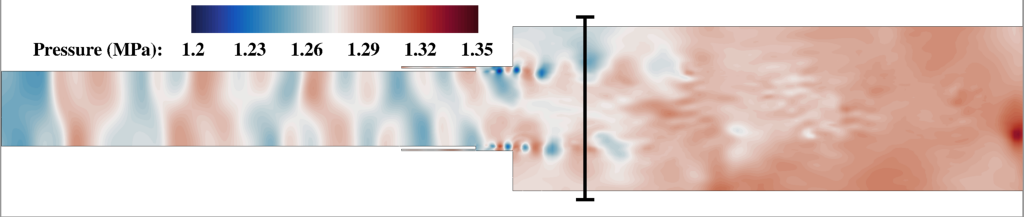
\includegraphics[width=0.84\linewidth,trim={0.5em 0.5em 0.5em 0.5em},clip]{Chapters/AdaptiveResults/Images/cvrc/fieldContours/fom_pressure_z.png}}
		\raisebox{-0.5\height}{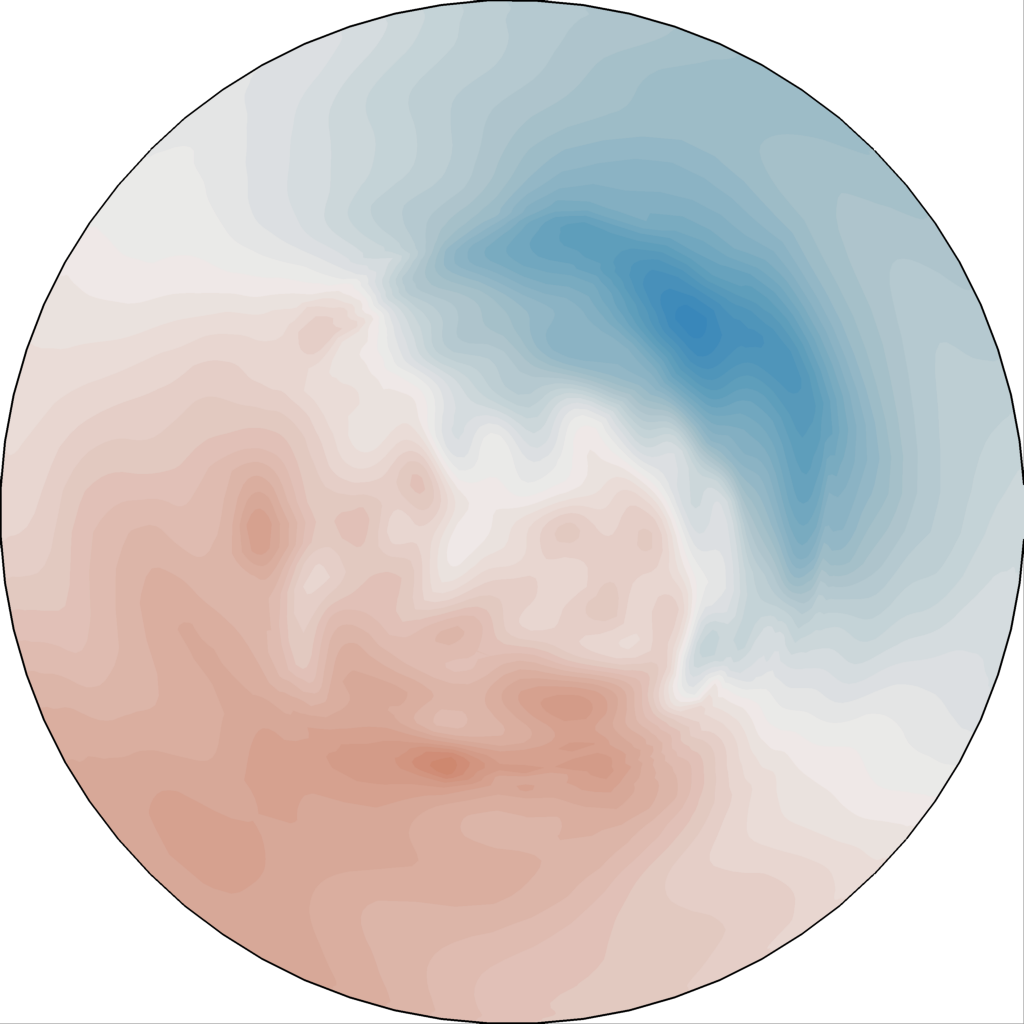
\includegraphics[width=0.14\linewidth,trim={0.0em 0.1em 0.0em 0.1em},clip]{Chapters/AdaptiveResults/Images/cvrc/fieldContours/fom_pressure_x.png}}
	\end{minipage}
    \begin{minipage}{0.99\linewidth}
		\raisebox{-0.5\height}{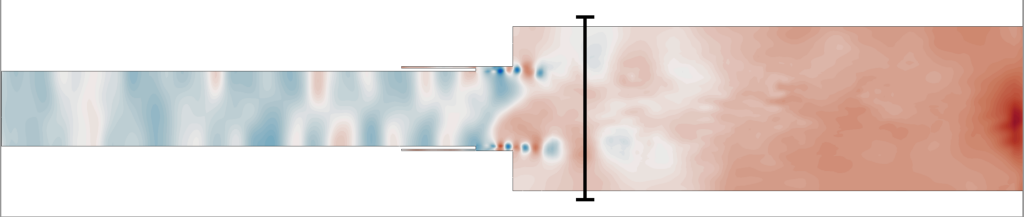
\includegraphics[width=0.84\linewidth,trim={0.5em 0.5em 0.5em 0.5em},clip]{Chapters/AdaptiveResults/Images/cvrc/fieldContours/proj_pressure_z.png}}
		\raisebox{-0.5\height}{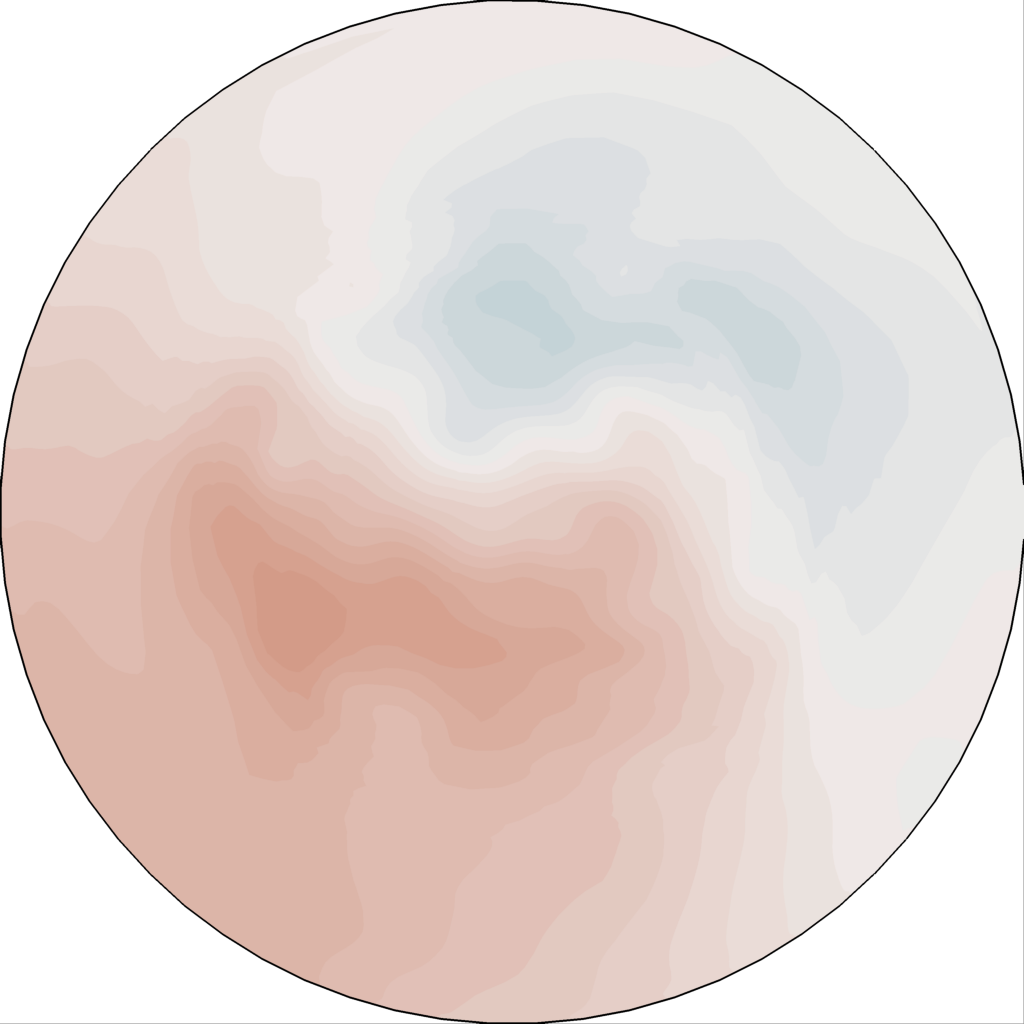
\includegraphics[width=0.14\linewidth,trim={0.0em 0.1em 0.0em 0.1em},clip]{Chapters/AdaptiveResults/Images/cvrc/fieldContours/proj_pressure_x.png}}
	\end{minipage}
    \caption{\label{fig:cvrcStaticPressureProjSlice}CVRC pressure field beyond training bounds, $\timeVar = 5.6$ ms, FOM at top and projected solution for $\numPrimModes = 100$ below.}
\end{figure}

\begin{figure}
	\begin{minipage}{0.99\linewidth}
		\raisebox{-0.5\height}{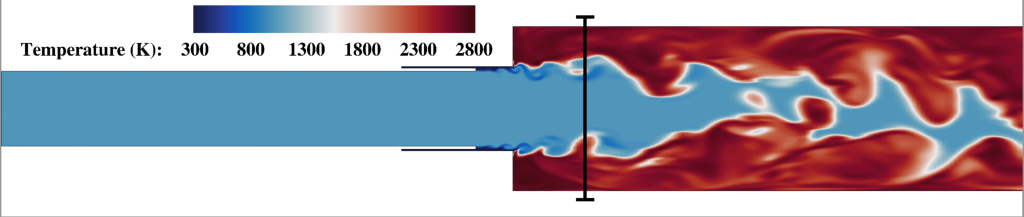
\includegraphics[width=0.84\linewidth,trim={0.5em 0.5em 0.5em 0.5em},clip]{Chapters/AdaptiveResults/Images/cvrc/fieldContours/fom_temperature_z.png}}
		\raisebox{-0.5\height}{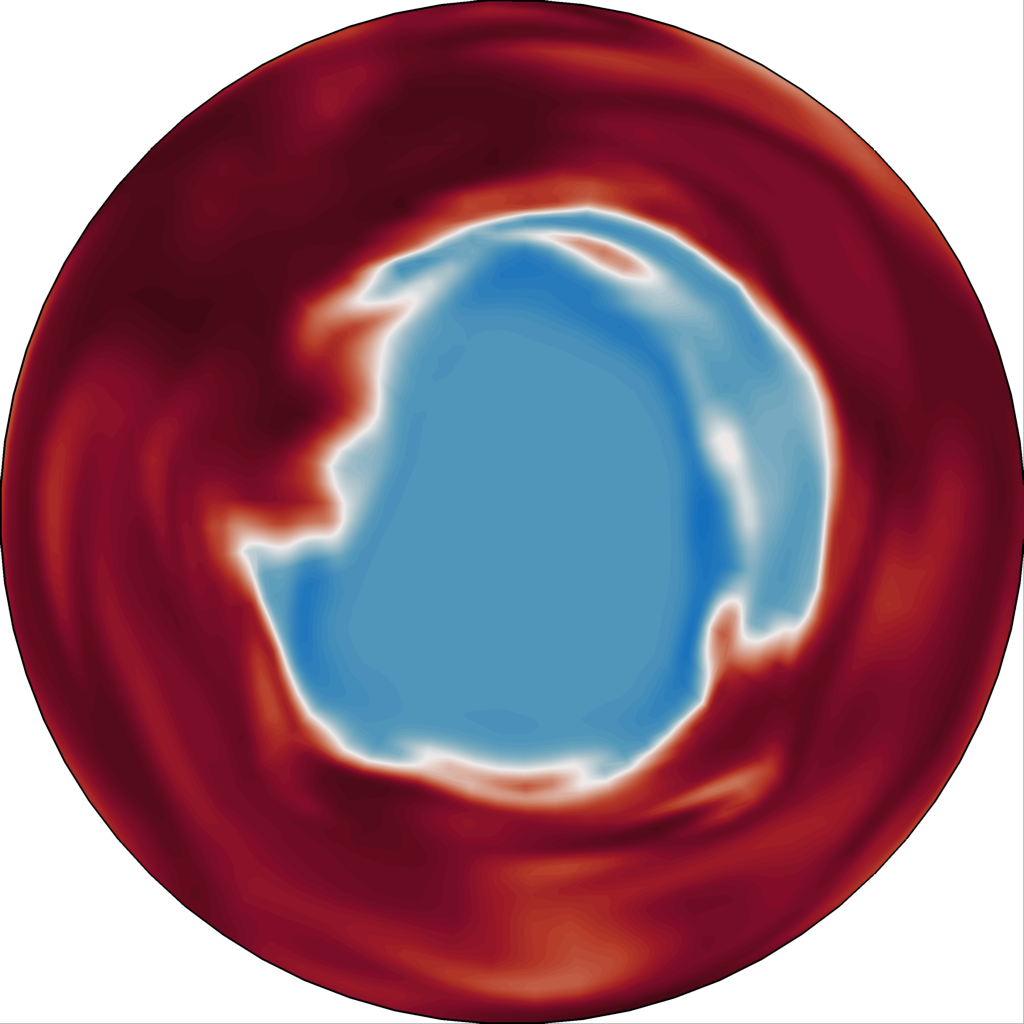
\includegraphics[width=0.14\linewidth,trim={0.0em 0.1em 0.0em 0.1em},clip]{Chapters/AdaptiveResults/Images/cvrc/fieldContours/fom_temperature_x.png}}
	\end{minipage}
    \begin{minipage}{0.99\linewidth}
		\raisebox{-0.5\height}{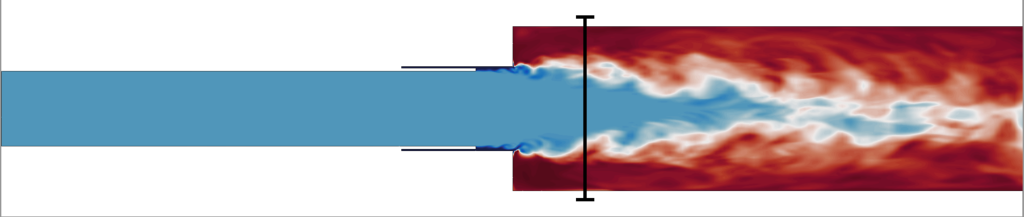
\includegraphics[width=0.84\linewidth,trim={0.5em 0.5em 0.5em 0.5em},clip]{Chapters/AdaptiveResults/Images/cvrc/fieldContours/proj_temperature_z.png}}
		\raisebox{-0.5\height}{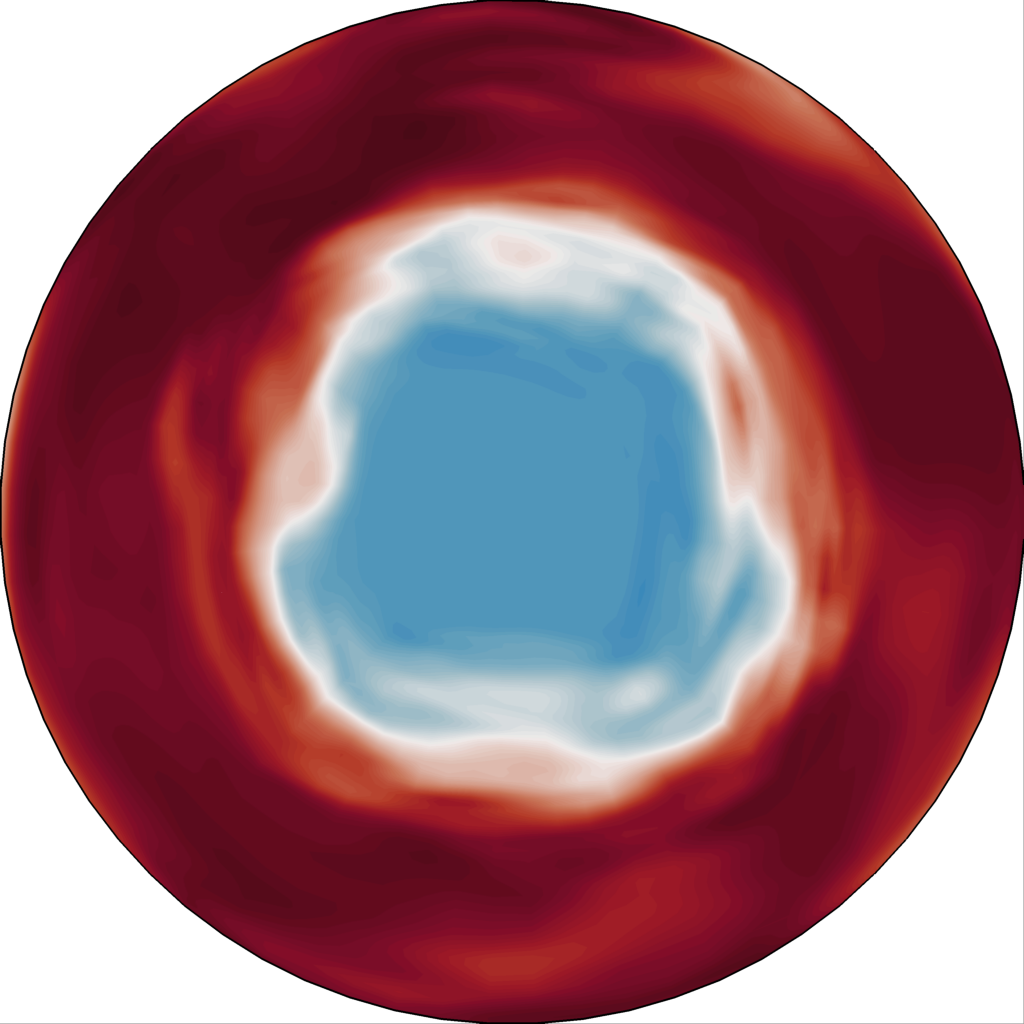
\includegraphics[width=0.14\linewidth,trim={0.0em 0.1em 0.0em 0.1em},clip]{Chapters/AdaptiveResults/Images/cvrc/fieldContours/proj_temperature_x.png}}
	\end{minipage}
    \caption{\label{fig:cvrcStaticTempProjSlice}CVRC temperture field beyond training bounds, $\timeVar = 5.6$ ms, FOM at top and projected solution for $\numPrimModes = 100$ below.}
\end{figure}

Given the poor performance of the unsampled PROM, it can be safely assumed that any HPROM will perform as poorly or worse. Ultimately, the failure lies purely with the fact that an accurate solution does not exist in the trial space. Alternatively, several methods have been proposed which \textit{adapt} a linear trial basis and hyper-reduction sampling configuration during the unsteady solution of the linear subspace PROM. Examples of approaches which propose time-variant trial bases include dictionary-based methods (sometimes referred to as \textit{local} bases)~\cite{Amsallem2012,Peherstorfer2014,Abgrall2016}, space-time trial bases~\cite{Choi2019,Hoang2022}, or basis transport maps~\cite{Iollo2014}. Although these methods have displayed exceptional accuracy improvements over static basis methods for convection-dominated problems, they still suffer from the fact that the constituent bases (e.g., those that form the dictionary) are constructed from the training data and may not accurately represent the unsteady solution when it significantly diverges from states observed in the full-order datasets. A notable exception is the work by Etter and Carlberg~\cite{Etter2019}, which updates the trial basis during online computations by vector space sieving.

The following sections explore adaptive PROMs by borrowing elements from the AADEIM framework by Peherstorfer~\cite{Peherstorfer2015,Peherstorfer2020Adaptive}, which leverages limited, periodic queries of the full-order model to incorporate the online state evolution in adapting the sampling configuration. This is investigated in combination with the recent one-step adaptation framework by Huang and Duraisamy~\cite{Huang2022a} as a method for adapting the trial basis.

% However, a promising alternative to dictionary approaches proposes online adaptation of the HPROM trial space and sample mesh using infrequent, judicious queries of the full-order model. The following section outlines trial space adaptation by the one-step basis adaptation method proposed by Huang \textit{et al.}~\cite{Huang2022a}, and adaptation of the HPROM sample mesh via a modification of the AADEIM approach by Peherstorfer~\cite{Peherstorfer2020Adaptive}.